% !TEX root = ../../main.tex
\begin{figure}[t!]
  \centering
  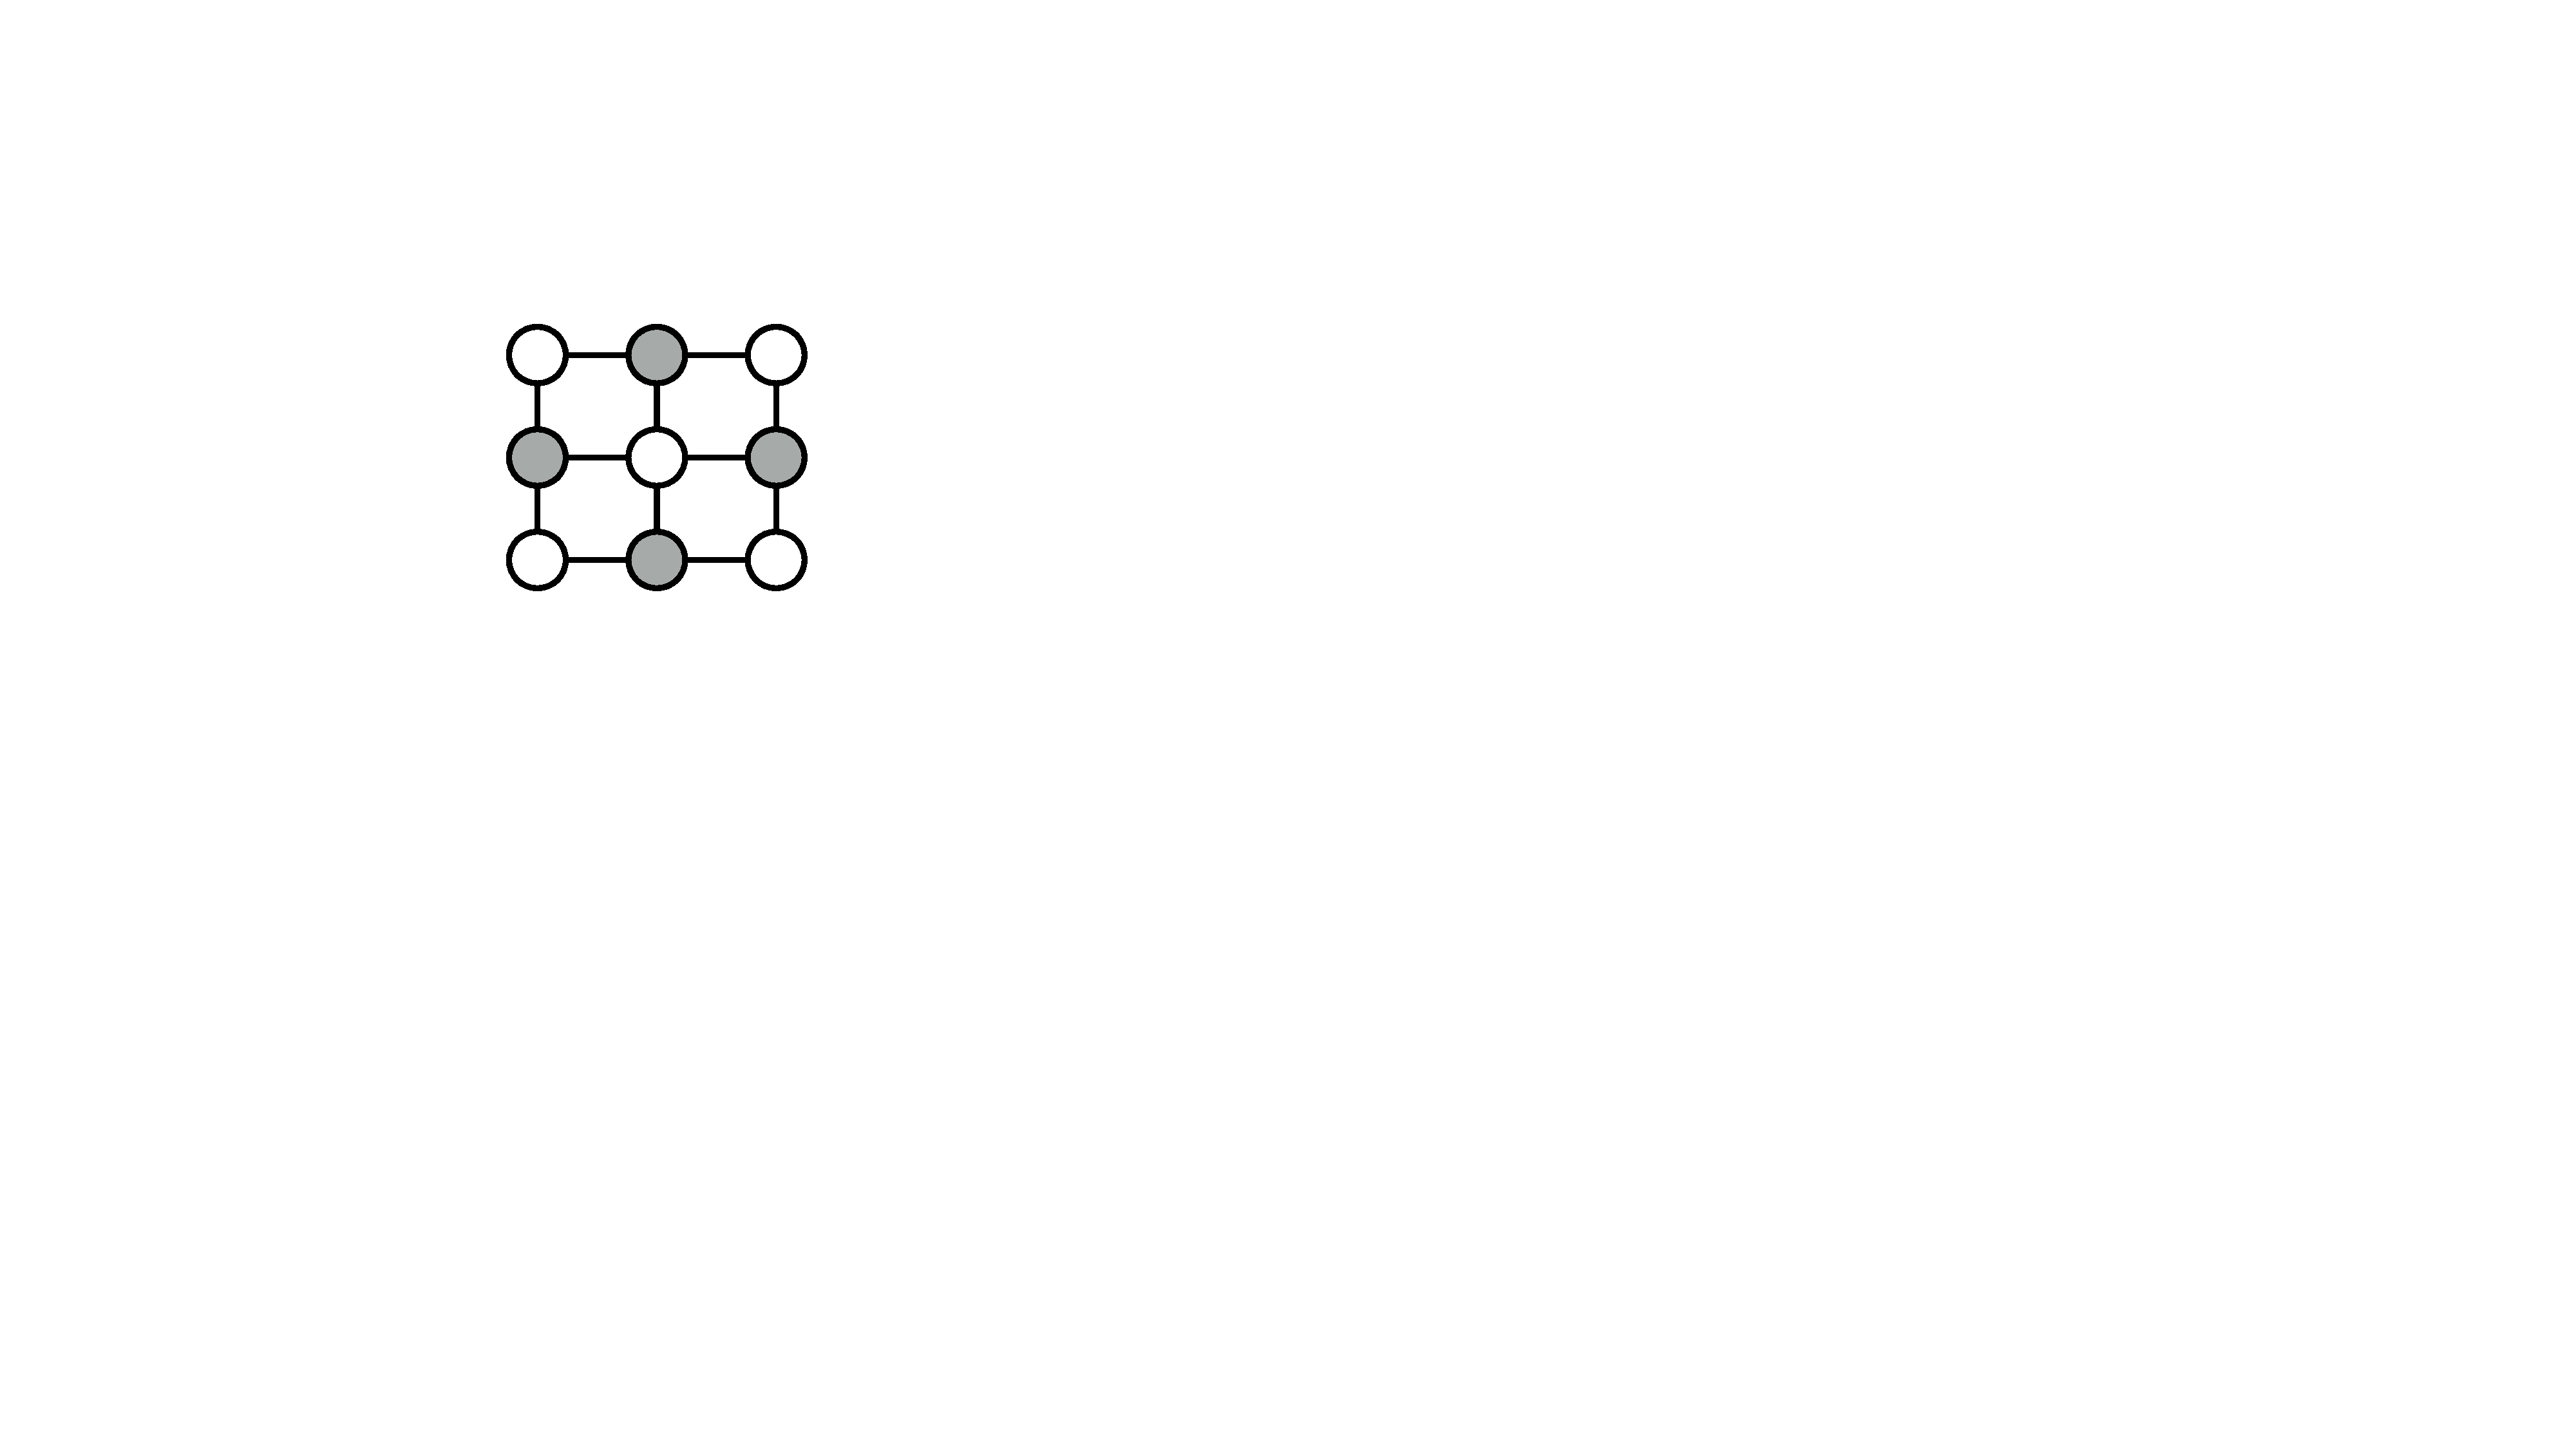
\includegraphics[height=0.2\paperheight]{ch-hvm/fig/markov-blanket-ising.pdf}
  \caption[Markov blanket of a random variable in an Ising model]{
  \textbf{The Markov blanket of a node in an Ising model consists of the node's nearest neighbors (nodes in the Markov blanket of the central node are shaded).} Conditioning on the Markov blanket of a node in a graphical model renders it conditionally independent of the rest of the variables. This enables building efficient variational approximations.}
  \label{fig:markov-blanket-ising}
\end{figure}